%! TEX root = tabulation.tex
\documentclass[11pt]{article}
\usepackage[margin=1.3in]{geometry}
\usepackage[utf8]{inputenc}
\usepackage[UKenglish]{babel}

%\usepackage[a4paper,
%            inner=20mm,
%            outer=50mm,% = marginparsep + marginparwidth
%                       %   + 5mm (between marginpar and page border)
%            top=20mm,
%            bottom=25mm,
%            marginparsep=5mm,
%            marginparwidth=60mm,
%            showframe% for show your page design, normaly not used
%            ]{geometry}
\usepackage{amsmath}
\usepackage{amsthm}
\usepackage{amsfonts}
\usepackage{amssymb}

\usepackage{tikz}
\usetikzlibrary{patterns}

\usepackage{authblk}
\usepackage{fullpage}
\usepackage{todonotes}
\usepackage{hyperref}
\usepackage{algorithm}
\usepackage[noend]{algpseudocode}
\usepackage{nameref}
\usepackage{cleveref}
%\usepackage[ruled,vlined,commentsnumbered,titlenotnumbered]{algorithm2e}

\DeclareMathOperator*{\E}{E}
\DeclareMathOperator*{\Var}{Var}

\newcommand{\floor}[1]{\lfloor {#1} \rfloor}
\newcommand{\bfloor}[1]{\big\lfloor {#1} \big\rfloor}
\newcommand{\bbfloor}[1]{\bigg\lfloor {#1} \bigg\rfloor}
\newcommand{\ceil}[1]{\lceil {#1}\rceil}
\newcommand{\Prp}[1]{\Pr\left[{#1} \right]}
\newcommand{\Ep}[1]{{\E}\left[{#1} \right]}
\newcommand\eps\varepsilon
\newcommand\Z{\mathbb Z}

\newtheorem {lemma} {Lemma}[section]
\newtheorem {fact} [lemma] {Fact}
\newtheorem {property} {Property}
\newtheorem {definition} {Definition}
\newtheorem {corollary} [lemma] {Corollary}
\newtheorem {theorem}[lemma] {Theorem}
\newtheorem {observation}[lemma] {Observation}
\newtheorem {question}{Question}[section]
\newtheorem {exercise}[question]{Exercise}

\newcommand{\unif}{\mathcal{U}}

% Drawing
\newcommand{\andtt}{ \mathbin{\texttt{\&}} }
\newcommand{\xor}{\oplus}
\newcommand{\ls}{ \mathbin{\texttt{<\!<}} }
\newcommand{\rs}{ \mathbin{\texttt{>\!>}} }


\renewcommand{\div}{\quad\text{div }}

\author{Thomas Dybdahl Ahle \and Jakob Bæk Tejs Knudsen}
\title{Engineering Hashing with Guarantees}
\begin{document}
\maketitle

\section{Introduction}

A new portable vector hash

Other hash functions:
Umash
Clhash
XXhash
Highway
Siphash
City, Farm, Wyhash, Murmur

Mention Mikkel's result about acc-0 not being strong enough to do hashing.
Bash Siphash a bit.

\section{Implementation}

In the following, $w$ is the word size and $b$ is a block size.
\begin{algorithm}[H]
   \caption{
      Main hash function:
      Let $x\in[2^{w\ell}]$.
      Let $a_i\in[2^w]$ be a list of $b$ random numbers,
      and let $\alpha\in[2^{61}-1]$ be random as well.
   }
   \begin{algorithmic}
      \State $h\gets \ell$
      \Comment{The first character is the length}
      \For{$i=0, b, 2b, \dots$}
         \State $b\gets \text{block-hash($x_i,\dots,x_{i+b-1}$)}$
         \Comment{Fixed length vector hash}
         \State $h\gets h\alpha + b \pmod{2^{61}-1}$
         \Comment{Variable length vector hash}
      \EndFor
      \For{$i=kb, kb+1, \dots, \ell$}
         \Comment{Handle last words}
         \State $h\gets h + (a_{i-kb} x_i \div 2^w)$
         \Comment{Simple fixed length vector hash}
      \EndFor
      \State \Return $\text{finalize-hash($h$)}$
   \end{algorithmic}
\end{algorithm}

For through-put the block-hash is the most important thing.
For latency, the remainder hash is the only the that matters.
We could in principle use a shorter version of the block-hash for the remainder,
but splitting it like this has the advantage that the block-hash can use heavy instructions that need instructor warm-up, without hurting our latency.

\begin{algorithm}[H]
   \caption{
      Tabulation finalizer:
      For $x\in[2^w]$, let $(x_1, \dots, x_c) = x$.
   }
   \begin{algorithmic}
      \State $h\gets 0$
      \For{$i=1, \dots, c$}
         \State $h\gets h \oplus T_i[x_i]$
      \EndFor
      \State \Return $h$
   \end{algorithmic}
\end{algorithm}

Other popular choices include Murmur and polynomial hashing.

In principle we could use the same randomness for 

\subsection{Fixed length vector hash (Mixing part 1)}

The point is to not have any collisions.
Any other concern is irrelevant at this step.

\paragraph{Multiply-Shift}
For $a_i\in[2^{2w}]$, $x_i\in[2^w]$
\[
   \sum_{i\in[n]} a_{i} x_i \div 2^{w}
\]
is universal.
In fact even
\[
   H(x_1, x_2) = x_1 + a x_2 \div 2^w
\]
is universal.

\paragraph{NH and PH}

\[
   \sum_{i\in[n]\text{, even}} (a_{i+1} + x_i \bmod 2^w)(a_i + x_{i+1} \bmod 2^w) \pmod{2^{2w}}
\]
\[
   \bigoplus_{i\in[n]\text{, even}} (a_{i+1} \oplus x_i)\odot(a_i \oplus x_{i+1})
\]

\paragraph{Vectorization}

Vector instructions allow us to perform NH very fast
\\
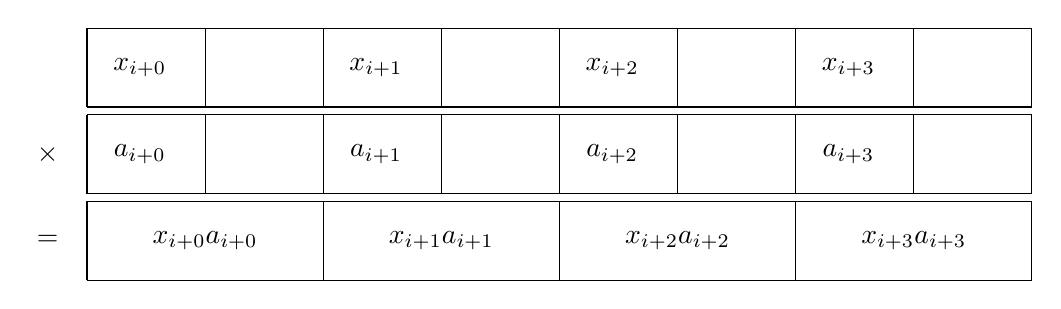
\begin{tikzpicture}
   % Horizontal lines
   \foreach \y in {0, -1.1, -2.2} {
      \draw (0, \y) -- (12, \y);
      \draw (0, \y-1) -- (12, \y-1);
   }
   % Vertical lines
   \foreach \y in {0, -1.1}
      \foreach \x in {0,1.5,...,12}
         \draw (\x, \y) -- (\x, \y-1);
   \foreach \x in {0,3,...,12}
      \draw (\x, -2.2) -- (\x, -3.2);
   % x =
   \node [draw=none] at (-.5, -1.6) {$\times$};
   \node [draw=none] at (-.5, -2.7) {$=$};
   % Numbers
   \foreach \x in {0,1,...,3} {
      \node [draw=none] at (3*\x+.67, -.5) {$x_{i+\x}$};
      \node [draw=none] at (3*\x+.67, -1.6) {$a_{i+\x}$};
      \node [draw=none] at (3*\x+1.5, -2.7) {$x_{i+\x}a_{i+\x}$};
   }
\end{tikzpicture}
\\
This picture shows the implementation of 
\[
   \sum_i a_ix_i
\]
By doing
\[
   \sum_i (a_i+x_i)(a_{i+1}+x_{i+1})
\]
we can process twice as many 32bit words per instruction.

\paragraph{AVX}
\paragraph{CL}
\paragraph{Alignment}


\paragraph{Prefetching}

As Lemire writes:
To prove the need for prefetch, optimize the code as much as possible, and only then show that prefetch makes a difference.
This is exactly what we have done.

Table of experiments

We follow XXHash and do prefetching for every other iteration of our inner loop.

\subsection{Variable length vector hash (Mixing part 2)}

Variable length hashing is one of the least well understood parts of hashing.
To our knowledge, there is only one commonly used approach.

In a given field over $\alpha$, define the polynomial:
\[h(x) = \sum_{i=1}^\ell x_i \alpha^i\]
Then $h(x)=h(y)$ exactly when
\[\sum_{i=1}^\ell (x_i-y_i) \alpha^i = 0.\]
Since a polynomial of degree $\ell$ can have at most $\ell$ zeros,
if we choose $\alpha$ uniformly at random in the field of size $p$,
the probability of a collision is $\ell/p$.

So we need a finite field.
There are two commonly used such fields: gallois and mod prime.
CLHash and Umash use gallois with a mod polynomial.

We use a Mersenne prime
with the lazy mod from the other paper.
CLHash and Umash use lazy mod polynomials as well.

Because the variable length hashing isn't done in the inner most loop,
the performance of the operation is not as important as the block-hash.
However, in principle there might be a way to do variable-length hashing as fast as block-hashing, in which case the block-hashing could be entirely cut from the hash function.


\subsection{Finalizing}

This is where we expect any strong properties of the hash function to be introduced.

\paragraph{Polynomial}
\paragraph{Murmur}
\paragraph{Tabulation}



\section{Seeding}

In recent years it has become popular for hash functions to take a secret seed
to help prevent constructed collision attacks.
In the theoretical community this has always been the approach to hash functions,
which can be understood only as functions randomly chosen from a given family.

While some hash functions use only a few random words for seeding, our uses about 2048.
This is well known to be necessary for many properties of strong hashing, such as concentration bounds.
\todo{Jakob, hjælp mig her}

   

\section{Counter Examples}

We present a number of counter examples (or attacks) on hash functions we have seen in the wild, or considered using our selves.

Counter-examples:
MUM
   - Based on mod 2^64-1
   - Based on clashes for a*x ^ a*y = b
   - men måske virker (a1 ^ x1)*(a2 ^ x2) ^ ... ?
   63(a ^ 64) ^ 65(a ^ 126) = 4032
   for alle ulige a 3..127.


   a1*a2 ^ (a1 ^ 30)*(a2 ^ 62)
   har nogle lidt sjove ting. F.eks. for a1=17 er der rigtigt mange a2 der virker.
   Vi har 17^30 = 15. Tilfælde?...
   Den værdi man kan få på mange måder er 992=1111100000. Dvs en del mindre end 128**2.

\paragraph{Mixing xor and multiplication}

It is often tempting to substitute xor of addition, since it guarantees we don't have do deal with overflows and carries.
For example, the MUM mixing function, which is also used in wyhash uses the following procedure:
\begin{algorithm}[H]
   \caption{
      MUM:
      Let $x_1,x_2\in [2^w]$ be a tuple to hash, and let $a_1,a_2\in[2^w]$ be uniformly random.
   }
   \begin{algorithmic}
      \State $h\gets (x_1 \oplus a_1)(x_2 \oplus a_2)$
      \State \Return $h \oplus (h >> 32)$
   \end{algorithmic}
\end{algorithm}
We can show that even without the final reduction from 64 to 32 bits, the above function can be tricked to produce many collisions.
Well, at least this one can:
\[
   h(x_1, x_2) = a_1 x_1 \oplus a_2 x_2.
\]
\begin{proof}
   We have a collision $(h(x_1,x_2) = h(y_1,y_2)$ exactly when
   \[
      a_1 x_1 \oplus a_1 y_1 = 
      a_2 x_2 \oplus a_2 y_2
      .
   \]
   Let $x_1=y_2 = 2^{w-1}-1$ and $x_2=y_1=2^{w-1}+1$.
   Then whenever $a_1$ and $a_2$ are both odd and $< 2^{w-1}$ both sides equal
   $2^{w+1}-1$.

   To see this, we focus on the left hand side.
   Let $a = a_1$ and $a = 2a' + 1$.
   Then we have $ax_1 = a 2^{w-1} - a$ and $ay_1 = a 2^{w-1} + a$.
   We use the following correspondence between negation and bit flipping:
\[
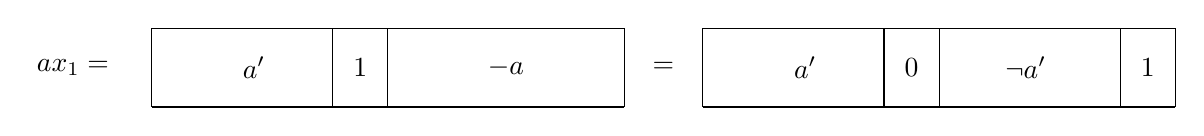
\begin{tikzpicture}
   \node [draw=none] at (-1, .5) {$ax_1 =$};
   \draw (0, 0) -- (6, 0);
   \draw (0, 1) -- (6, 1);
   \draw (0, 0) -- (0, 1);
   \draw (3, 0) -- (3, 1);
   \draw (6, 0) -- (6, 1);
   \draw (2.3, 0) -- (2.3, 1);
   \node [draw=none] at (2.65, .5) {$1$};
   \node [draw=none] at (1.3, .5) {$a'$};
   \node [draw=none] at (4.5, .5) {$-a$};

   \node [draw=none] at (6.5, .5) {$=$};
\draw (7, 0) -- (13, 0);
   \draw (7, 1) -- (13, 1);
   \draw (7, 0) -- (7, 1);
   \draw (10, 0) -- (10, 1);
   \draw (13, 0) -- (13, 1);
   \draw (9.3, 0) -- (9.3, 1);
   \draw (12.3, 0) -- (12.3, 1);
   \node [draw=none] at (8.3, .5) {$a'$};
   \node [draw=none] at (9.65, .5) {$0$};
   \node [draw=none] at (11.1, .5) {$\neg a'$};
   \node [draw=none] at (12.65, .5) {$1$};
\end{tikzpicture}
\]
Now
\[
\begin{tikzpicture}[margin=2em]

   \draw (7,    2.2) -- (13,   2.2);
   \draw (7,    3.2) -- (13,   3.2);
   \draw (7,    2.2) -- (7,    3.2);
   \draw (10,   2.2) -- (10,   3.2);
   \draw (13,   2.2) -- (13,   3.2);
   \draw (9.3,  2.2) -- (9.3,  3.2);
   \draw (12.3, 2.2) -- (12.3, 3.2);
   \node [draw=none] at (8.3,   2.7) {$a'$};
   \node [draw=none] at (9.65,  2.7) {$0$};
   \node [draw=none] at (11.1,  2.7) {$\neg a'$};
   \node [draw=none] at (12.65, 2.7) {$1$};

   \node [draw=none] at (6.5, 1.6) {$\oplus$};

   \draw (7, 1.1) -- (13, 1.1);
   \draw (7, 2.1) -- (13, 2.1);
   \draw (7, 1.1) -- (7, 2.1);
   \draw (10, 1.1) -- (10, 2.1);
   \draw (13, 1.1) -- (13, 2.1);
   \draw (9.3, 1.1) -- (9.3, 2.1);
   \draw (12.3, 1.1) -- (12.3, 2.1);
   \node [draw=none] at (8.3, 1.6) {$a'$};
   \node [draw=none] at (9.65, 1.6) {$1$};
   \node [draw=none] at (11.1, 1.6) {$a'$};
   \node [draw=none] at (12.65, 1.6) {$1$};

   \node [draw=none] at (6.5, .5) {$=$};

   \draw (7, 0) -- (13, 0);
   \draw (7, 1) -- (13, 1);
   \draw (7, 0) -- (7, 1);
   \draw (10, 0) -- (10, 1);
   \draw (13, 0) -- (13, 1);
   \draw (9.3, 0) -- (9.3, 1);
   \draw (12.3, 0) -- (12.3, 1);
   \node [draw=none] at (8.3, .5) {$0$\dots};
   \node [draw=none] at (9.65, .5) {$1$};
   \node [draw=none] at (11.1, .5) {$1\dots$};
   \node [draw=none] at (12.65, .5) {$0$};
\end{tikzpicture}
\]
which is equal to $2^{w+1}-1$ independent of the choice of $a$.
\end{proof}

\subsection{Empty Buckets}

We add a new test to SMHasher

\end{document}
